\documentclass[msc,proposal,hidelot,hideabstract]{ppgccufmg} % ou [msc] para dissertações
										% de mestrado. Para propostas ou
										% projetos, usar [phd,project],
										% [msc,proposal], etc.
\usepackage[brazil]{babel} % ajusta vários detalhes para
						   % documentos escritos em português,
						   % principalmente hifenização
\usepackage[T1]{fontenc}   % permite a hifenização de
						   % palavras acentuadas
\usepackage[utf8x]{inputenc} % ou [utf8x] para quem prefere
							 % usar a codificação UTF-8
\usepackage{graphicx} % define o comando \includegraphics
					  % para a inclusão de figuras
\usepackage[square]{natbib} % permite citações naturalmente
							% integradas ao texto
\usepackage[a4paper,
portuguese,
bookmarks=true,
bookmarksnumbered=true,
linktocpage,
colorlinks=true,
citecolor=black,
urlcolor=black,
linkcolor=black,
filecolor=black,
]{hyperref}
\usepackage[table,xcdraw]{xcolor}


\begin{document}
\ppgccufmg{
title={Uma linguagem para modelagem conceitual em XBRL},
author={Vagner Clementino},
university={Universidade Federal de Minas Gerais},
course={Ciência da Computação},
address={Belo Horizonte},
date={2015-05},
advisor={Rodolfo F. Resende},
abstract={Resumo}{resumo},
}
\chapter{Introdução}
\label{ch:Contexto}
No cenário atual, onde os sistemas de informação tem se tornado grandes e complexos, vemos a existência de um ecossistema de sistemas, também conhecidos como \textit{System of System} (SoS) \cite{Nakagawa:2013:SAF:2489850.2489853}. Organizações de grande porte, como os governos nacionais, precisam projetar sistemas de sistema ao invés vez de sistemas isolados a fim de enfrentar desafios tais como: $(i)$ colaboração entre organizações financiadas e geridas de forma independente; $(ii)$ migração para um ambiente orientado a serviços (SOA\footnote{Service Oriented Architecture }); $(iii)$ processos de testes e verificação da conformidade para sistemas de sistemas. Neste contexto, surge a necessidade do desenvolvimento de \textit{abordagens, técnicas e tecnologias} para a interação e evolução dos SoS.
     
No tocante a interoperabilidade de dados, diversos padrões vêm sendo propostos. Mais recentemente o formato JSON \cite{RFC4627} vêm crescendo em popularidade, contudo, o intercâmbio de dados é realizado primordialmente através da XML (Extensible Markup Language\footnote{\url{http://www.w3.org/XML/}}) e seus derivados. Na área medica, o padrão HL7 V3 message\footnote{\url{http://www.hl7.org/}} vêm sendo largamente adotado para troca de mensagem entre sistemas médicos \cite{Andrikopoulos:2013:TEO:2491845.2491890}{}. No contexto dos Sistemas de Informação Geográficas (SIG) a GML (Geography Markup Language\footnote{\url{http://www.opengeospatial.org/standards/gml}}) consolidou-se com o principal instrumento para interoperabilidade de dados geográficos \cite{gmlpaper}{}. Na área financeira diversas linguagens de marcação vêm sendo utilizadas para o intercâmbio de informações na Internet: \textit{Open Financial Exchange}\footnote{\url{http://www.ofx.net/}} (OFX), \textit{Eletronic Business Using XML}\footnote{\url{http://www.ebxml.org}} (ebXML), \textit{Financial Information eXchange}\footnote{\url{https://fixspec.com/}} (FIX), \textit{Market Data Definition Language}\footnote{\url{http://www.mddl.org}}, dentre outras \cite{xbrl_conceitos_aplicacoes}{}.

Com o advento da Web as linguagens de marcação cresceram em importância sobretudo devido a necessidade de se adicionar significado a informações sendo transferidas. Contudo, o padrão HTML (Hypertext
Markup Language) foi desenvolvido com objetivo de descrever \textit{como} a informação deve ser apresentada e não possui qualquer compromisso com o significado da informação. Nos meados da década de 1980,  a Organização para Padronização Internacional (ISO) propôs uma metalinguagem padrão a fim de etiquetar informações com conteúdo semântico. Esta linguagem foi denominada como \textit{Standard Generalized Markup Language} (SGML) \cite{smith1988sgml}.

A linguagem SGML, embora fosse capaz de definir diferentes tipos de marcação, a sua flexibilidade trouxe como preço a complexidade. O conceito era correto, todavia, havia a necessidade de ser mais simples. Com este objetivo em mente, um pequeno grupo de trabalho e um maior número de interessados começou a trabalhar em
meados dos anos 1990 em um subconjunto de SGML conhecido como \textit{Extensible Markup Language} (XML). A primeira versão foi publicada em 1996 e, dois anos mais tarde, o World Wide Web Consortium\footnote{\url{http://www.w3.org}} (W3C) publicou uma versão revisada \cite{Fawcett:2012:BX:2408362}{}.

Conforme exposto, a XML foi especificada a partir da SGML, na tentativa de se resolver as limitações da HTML
e da SGML. Neste sentido, um documento em XML pode ser publicado na Web, interpretado por pessoas
ou processado por aplicações. Apropriando-se desta características da XML, diversos linguagens vêm sendo propostas com a finalidade de troca de informações.

A XBRL (\textit{eXtensible Business Reporting Language}) é uma linguagem para divulgação e intercâmbio de informações financeiras baseada em XML (\cite{xbrl_conceitos_aplicacoes}). O padrão vem sendo adotado por diversas instituições e empresas em todo mundo com o suporte de um consórcio global\footnote{\url{www.xbrl.org}} com mais de 650 membros que incentivam a criação de jurisdições locais. Atualmente o consórcio conta com 24 jurisdições, sendo que em países como  Estados Unidos, Grã-Bretanha e Austrália, a XBRL já é a linguagem oficial para entrega de relatórios à órgãos de governo. A figura \ref{fig:world_map} exibe os países que estão promovendo a adotação da XBRL.

\begin{figure}[hbtp]
\centering
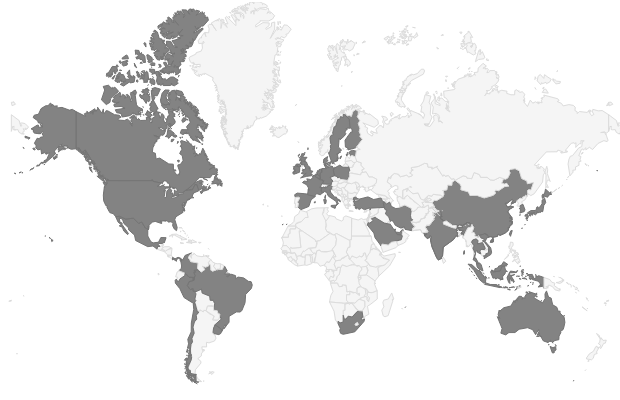
\includegraphics[width=.75\textwidth]{img/world-map.png}
\caption{O uso da XBRL no mundo}
\label{fig:world_map}
\end{figure}

Os estudos para definição da XBRL iniciaram em 1998 nos Estados Unidos pelo contador Charles Hoffman com apoio \textit{Institute of Certified Public Accountants} (AICPA). O objetivo era utilizar a XML padronizar a divulgação de informações financeiras em formato eletrônico. A primeira versão do padrão, a XBRL 1.0, foi lançada em 2000, sendo a versão 2.0 lançada em dezembro de 2001. No mês de dezembro de 2003, foi lançada a versão 2.1 (\cite{hoffman_2006}), corrigindo algumas deficiências detectadas na versão anterior. A versão 2.1 se mantêm como a versão mais atual e estável da XBRL.

A linguagem XBRL define a estrutura básica dos documentos de instância, que são aqueles que portam os dados, e possibilita ainda a especificação de taxonomias que podem ser criadas para acomodar particularidades de cada organização por meio da introdução de novos elementos, denominados conceitos. Neste sentido, a linguagem possui elementos que facilitam a sua extensão e, por consequência, a adoção em diversos contextos.

Apesar de sua crescente adoção, falta à XBRL uma notação que facilite a sua modelagem e a comunicação entre os diferentes \textit{stakeholders}. A necessidade de um modelo abstrato para a XBRL foi manifestada pelo próprio \textit{XBRL Consortium}. Em 2010 (\cite{xbrl_preserve_promote_particite}), o consórcio declarou que a criação de um modelo conceitual é uma das seis iniciativas que darão suporte a contínua adoção do padrão. Com o objetivo de preencher esta lacuna propõe neste documento o desenvolvimento de uma linguagem conceitual para a XBRL. A seguir descreve-se como o documento está estruturado.

No Capítulo \ref{ch:justificativa} discute-se as justificas para adoção da XBRL bem como da criação de uma linguagem conceitual. O Capítulo \ref{ch:revisao} apresenta-se a revisão da literatura no tocante a criação de ontologias em diversos campos dos conhecimento, especialmente para área financeira e contábil. No Capítulo \ref{ch:metodologia} é discutida a metologia a ser aplicada. No Apêndice \ref{attch:cronograma} é exibido o cronograma do trabalho.

\chapter{Justificativa}
\label{ch:justificativa}

Nas organizações as informações contábeis e financeiras são armazenadas em diversos formatos (planilhas eletrônicas, documentos de texto, bancos de dados relacionais e etc). Não obstante, se faz necessário a transformação destas informações em um formato único a fim de facilitar a sua recuperação bem como a sua transmissão para outros sistemas. O processo de transformação e redirecionamento da informação internamente na organização, entre a organização e sua filiais ou mesmo entre a empresa e os governos. Este fluxo de informação, especialmente para a geração de relatórios, é exibido na figura \ref{fig:fluxo_dados}.

\begin{figure}[hbtp]
\centering
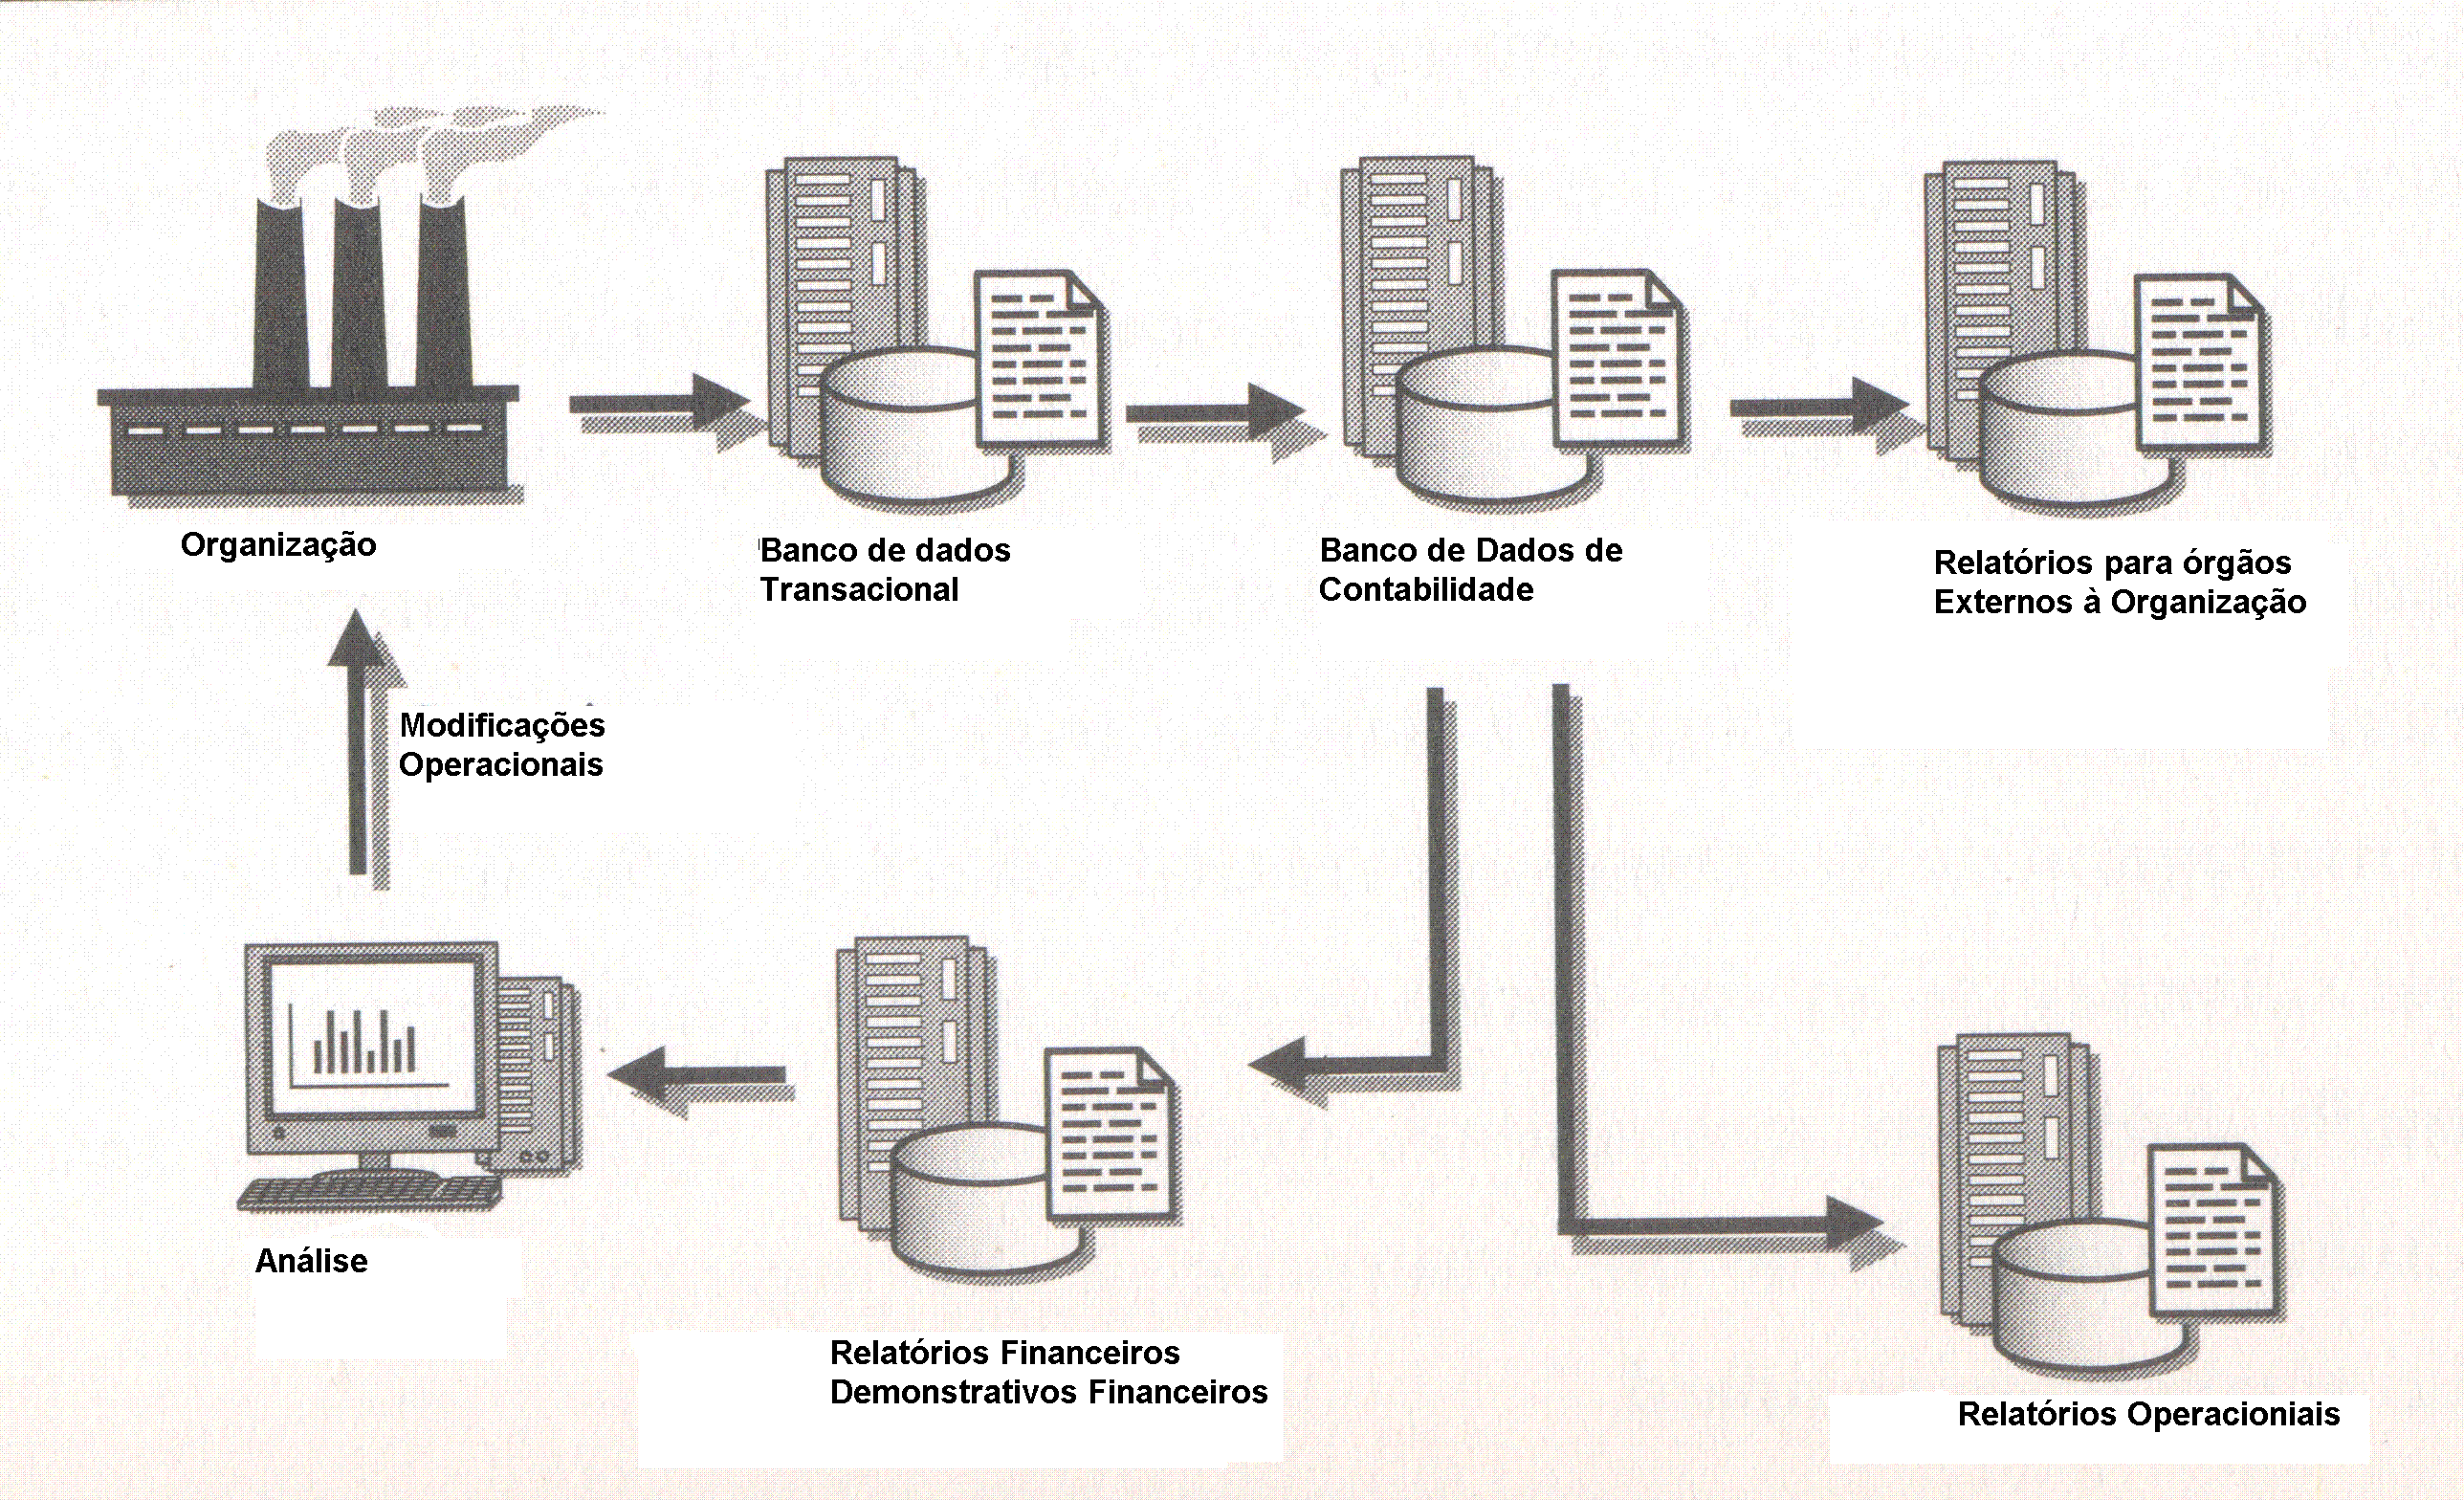
\includegraphics[width=.75\textwidth]{img/fluxo_informacoes.png}
\caption{Fluxo de dados financeiros em uma organização. Adaptado de (\cite{bergeron2004essentials}).}
\label{fig:fluxo_dados}
\end{figure}

Se pensarmos em uma organização que necessitem receber informações de diversos locais, como por exemplo o governo federal de uma país que solicite a prestação de contas de estados e municípios, onde cada ente possui seu próprio sistema para registro dos fatos financeiros. Neste contexto, haverá a necessidade de se criar diferentes interfaces para a conversão de formatos e padrões de contabilização. A figura \ref{fig:interfaces} ilustra este cenário.


\begin{figure}[hbtp]
\centering
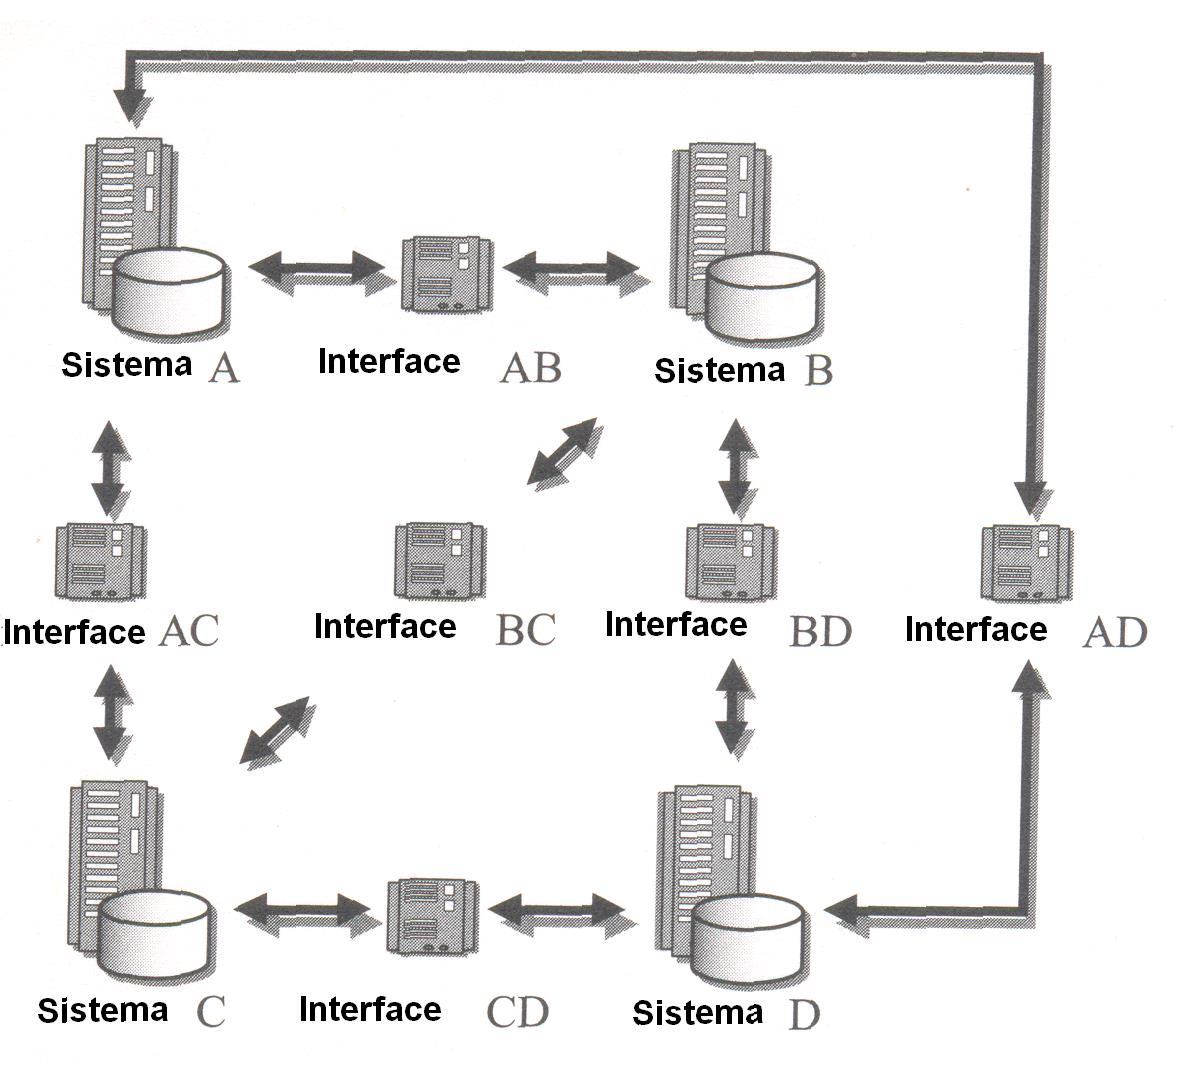
\includegraphics[width=.75\textwidth]{img/interfaces.png}
\caption{Diferentes interfaces para a interoperabilidade entre sistemas. Adaptado de (\cite{bergeron2004essentials}).}
\label{fig:interfaces}
\end{figure}

A solução utilizada para minimizar estes problemas é adoção de uma linguagem de marcação que facilite o intercâmbio e apresentação na Internet, bem como proporcione o armazenamento em qualquer base de dados. Neste sentido a XBRL vêm sendo adotado como padrão em diversos países. O processo de troca de informações financeiras é simplificado pela XBRL tendo em vista que a transformação da informação original é realizada uma única vez para o formato XBRL. Posteriormente a informação poderá ser reutilizada e/ou distribuída automaticamente para diversos outros formatos. A figura \ref{fig:fluxo_info_xbrl} exibe a simplificação na troca de informação com a adoção do XBRL.

\begin{figure}[hbtp]
\centering
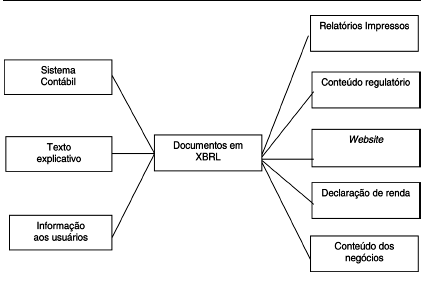
\includegraphics[width=.75\textwidth]{img/fluxo_info_xbrl.png}
\caption{Melhoria no fluxo de informação com XBRL. Adaptado de (\cite{hoffman2001xbrl}).}
\label{fig:fluxo_info_xbrl}
\end{figure}

Apesar de sua importância e crescente adoção, o \textit{XBRL Consortium} sentiu a necessidade de definir um modelo abstrato da XBRL (\cite{xbrl_preserve_promote_particite}) que facilitasse a compreensão da linguagem pelos profissionais da tecnologia da informação.Em 2012 foi proposto o \textit{XBRL Abstract Model 2.0}\footnote{\url{http://www.xbrl.org/Specification/abstractmodel-primary/PWD-2012-06-06/abstractmodel-primary-pwd-2012-06-06.html}} que consiste basicamente de uma versão estendida da UML com objetivo de captura aspectos semânticos da XBRL. 

Um modelo abstrato deverá remover do seu escopo qualquer questão relativa à implementação do objeto modelado. Neste sentido, no caso de XBRL, o modelo abstrato deveria remover todas as referências a XML, o que não ocorreu no XBRL Abstract Model. Ademais, apesar da UML ser largamente utilizada entre os profissionais de Tecnologia da Informação, o seu uso para comunicação com os demais stakeholders muitas vezes não é o ideal (\cite{peixoto2008comparison}).

Neste contexto se faz necessário a proposição de linguagem conceitual para a XBRL com as seguintes características:
 \begin{itemize}
 	\item Não contenha questões relativa ao XML
 	\item Possibilite o desenho de aplicações que utilizem a XBRL
 	\item Facilite a comunicação entre os diversos stakeholders envolvidos no domínio da XBRL.
 \end{itemize}
 
No próximo capítulos iremos revisar a literatura relativo à definição de ontologias, especialmente no domínio contábil/financeiro.

\chapter{Revisão da Literatura}
\label{ch:revisao}

\cite{Bosch:2013:APD:2575980.2575988} apresentam um estudo sobre a criação de ontologias com base em XML Schemas. Arquivos no formato XML Schemas são utilizados por linguagem como XBRL para definir os conceitos a serem utilizados em determinado domínio.Neste sentido, todas as informações localizadas m XML Schemas podem ser reutilizados a fim de reduzir a necessidade de criar ontologias de domínio a partir do zero. Os autores argumentam que o tempo e esforço economizado poderiam ser utilizados para acrescentar informações semânticas específicas do domínio específico, tendo em vista que este tipo de detalhamento não existem nos XML Schemas.

Em \cite{journals/ijcsa/Pierre08} há uma discussão sobre alguns dos problemas do uso de representações formais no domínio da contabilidade. O objetivo do autor era construir uma representação das informações financeiras de uma forma eficiente. Todavia, devido a própria maneira que a contabilidade é construída, basicamente de leis e normas, existem diversos problemas na representação dos elementos da mesma. Não obstante, Pierre considera a XBRL como uma boa alternativa para uma representação formal da contabilidade. O autor ressalta que a XBRL trouxe novos elementos para o processo de criação de relatórios financeiros: $(i)$ facilidade na produção e publicação das informações contábeis; $(ii)$ compartilhamento e possibilidade comparação partilha de informação; $(iii)$ verificação e certificação da informação; $(iv)$ ganho no processo de análise. Ele conclui que XBRL é bom padrão para armazenar informações, contudo, faz uma crítica ao padrão por não fornecer nenhuma formalização explícita de dados financeiros ou das normas contabilísticas.

\cite{lupacsc2010role} realiza uma análise do REA Framework\footnote{\url{http://reatechnology.com/}} como uma ontologia de contabilidade para sistemas de informação. Os elementos básicos do REA são recursos, eventos, agentes, fluxos, controle e \textit{duality} (\cite{mccarthy1982rea}). Os autores estendem o REA a fim de possibilitar a adição e compartilhamento do conhecimento.

\cite{gailly2007positioning} utilizaram a UML para representar graficamente ontologias baseadas no REA. Os autores utilizaram metodologias tradicionais para a criação de ontologias para desenvolver o modelo proposto e argumentam que REA é uma ontologia de domínio do negócio. Eles concluem que linguagens conceituais tais como UML possuem a riqueza necessária para representar REA componentes ontológicos. Todavia, alguns detalhes dos elementos representados não são capazes de serem explicitados.

\cite{sugumaran2002ontologies} discutem a criação, uso e gestão de ontologias para modelagem conceitual. Eles também propõe um processo para gestão de ontologias. Os objetivos dos trabalho incluem demostrar a importância de ontologias na modelagem conceitual e propor um modelo baseada em heurística  para a criação de ontologias em determinado domínio. Eles observam que a maioria das ontologias são criadas manualmente e que não existe uma metodologia largamente aceita para construção das mesmas. O seu método de criação ontologia proposto é composto por quatro etapas. O primeiro passo é a identificação de termos básicos do domínio. Isto inclui duas subetapas: a identificação dos termos mais frequentes e a identificação de sinônimos e termos relacionados. O segundo passo é a identificação dos relacionamentos. Existem três tipos de relações: relações entre termos básicos, relações entre ontologias, e as relações entre ontologias e sub-ontologias. O terceiro passo é a identificação de restrições e regras do domínio. O quarto passo é a identificação de restrições de nível superior. Estas restrições capturar o conhecimento de domínio. Os autores observam ainda que, enquanto a maioria das ontologias são construídos estaticamente, a maioria dos domínios, na verdade, evoluem com o tempo. O desenvolvimento de uma ontologia deve incluir esta evolução.

\chapter{Metodologia}
\label{ch:metodologia}

O processo de desenvolvimento deste trabalho pode ser dividido em quatro partes principais: $I$\textit{ - Revisão Sistemática da Literatura}; $II$\textit{ - Desenvolvimento da Linguagem}; $III$\textit{ - Construção da Ferramenta}; $IV$\textit{ - Avaliação}. Cada uma das etapas é detalhada nas próximas seções.

\section{Revisão Sistemática}
\label{sec:revisao_sistematica}

O primeiro passo no desenvolvimento do trabalho será revisar a literatura relativa a criação de ontologias, especialmente no domínio contábil/financeiro. Conforme proposto por \cite{wohlin2012experimentation} será definido um protocolo de revisão com o objetivo de conduzir o processo de coleta de artigos. Este protocolo conterá, dentre outros tópicos, os critérios de seleção de trabalhos, estratégia para extração de dados;definição de questões de pesquisas, dentre outros. O protocolo será revisto com o orientador visando garantir suas consistência e validade.

Nesta etapa também será revisada a especificação da XBRL\footnote{\url{http://specifications.xbrl.org/specifications.html}} com o objetivo de conseguir subsídios para a criação da ontologia. Conforme discutido em \cite{lupacsc2010role}{}, um dos passos para criação de uma ontologia efetiva é a identificação de termos básicos do domínio. Nesta tarefa poderá utilizado técnicas de recuperação da informação como índices invertidos (\cite{baeza1999modern}).

\section{Desenvolvimento da Linguagem}
\label{sec:dese_lingugem}

Finalizado o levantamento teórico do trabalho, o próximo passo é definir os elementos da linguagem. Por se tratar de uma linguagem conceitual visando a facilitar modelagem e a comunicação da XBRL, nesta fase será construído os elementos gráficos da linguagem. Tais elementos irão se apropriar dos objetos de linguagens como a UML e a BPMN, contudo, fornecendo primitivas adequadas para a representação dos dados contábeis e financeiros.

\section{Ferramenta de Modelagem}
\label{sec:ferramenta}

A adoção de uma nova notação será facilitada se existirem ferramentas que facilitem a sua criação, alteração e disponibilização. Neste sentido, faria pouco sentido definir uma linguagem conceitual para a XBRL sem, contudo, criar uma ferramenta que lhe desse apoio. Assim, uma das etapas deste trabalho será o desenvolvimento de uma ferramenta que possibilite a criação de diagrama no modelo proposto. Esta ferramenta será de suma importância na última etapa do trabalho, que trata da avaliação da linguagem proposta.

\section{Avaliação}
\label{sec:avaliacao}

A fim de avaliar se a linguagem proposto atendeu aos seus requisitos, será realizadas uma bateria de testes com diferentes usuários. O baseline será o \textit{XBRL Abstract Model}, onde pretende-se analisar fatores como capacidade de comunicação, expressividade, dentre outros aspectos das duas linguagens.

O experimentos de avaliação será composto de duas etapas. Em um primeiro momento, profissionais de tecnologia da informação e contabilidade, serão convidados a modelar uma taxonomia XBRL utilizando a linguagem proposta e o XBRL Abstract Model. Posteriormente, estes diagramas serão avaliados por outros profissionais no tocante as aspectos como expressividade. Estes dados serão tabulados para posterior avaliação.

% Incluindo bibliografia:
\ppgccbibliography{./bib/bibliografia}
% apêndices, se houver
%\begin{appendices}
%\chapter{Um apêndice}
%...conteúdo do apêndice...
%\chapter{Outro apêndice}
%...conteúdo do apêndice...
%\end{appendices}
% anexos, se houver
\begin{attachments}
\chapter{Cronograma}
\label{attch:cronograma}

\begin{table}[h]
\begin{tabular}{|c|l|c|c|}
\hline
\rowcolor[HTML]{C0C0C0} 
\textbf{\#} & \multicolumn{1}{c|}{\cellcolor[HTML]{C0C0C0}\textbf{Atividade}} & \textbf{Início (MM/AAAA)} & \textbf{Termino  (MM/AAAA)} \\ \hline
01          & Revisão da literatura                                           & 07/2015                   & 08/2015                     \\ \hline
02          & Revisão da especificação XBRL                                   & 09/2015                   & 09/2015                     \\ \hline
03          & Definição da linguagem                                          & 10/2015                   & 12/2015                     \\ \hline
04          & Construção da ferramenta                                        & 01/2016                   & 02/2016                     \\ \hline
05          & Avaliação da linguagem                                          & 03/2016                   & 03/2016                     \\ \hline
06          & Redigir a dissertação                                           & 04/2015                   & 05/2016                     \\ \hline
07          & Defesa da dissertação                                           & 07/2016                   & 07/2016                     \\ \hline
\end{tabular}
\label{tab:cronograma}
\end{table}

\end{attachments}
\end{document}